\documentclass[xcolor=pdftex,dvipsnames]{beamer}

\usepackage{amsmath}
\usepackage{amssymb}
\usepackage{comment}
\usepackage{textcomp}

\DeclareRobustCommand{\rsout}[1]{\texorpdfstring{\sout{#1}}}

\title{Microeconomic Theory --- ECON 323 503 \\ Chapter 13: Game Theory}
\author{Vikram Manjunath}       %
\institute{Texas A\&M University}
\setbeamertemplate{navigation symbols}{}
\setbeamertemplate{footline}{}
\usefonttheme{serif}
\begin{document}

\maketitle

\begin{frame}
\frametitle{Outline}
\begin{enumerate}[<+->]
\item  Static games: a one-off interaction between players where they choose their actions at the same time.
\item Dynamic games: players either make their choices one after another or they interact repeatedly.
\item Auctions: a common way of selling goods. It ends up being a ``game'' played between bidders.
\end{enumerate}
\end{frame}


\begin{frame}
  \frametitle{Static games}  
  Two airlines $U$ and $A$.

  \bigskip
\uncover<2->{  Each picks the number flights (how many passengers) to fly between
  LA and Chicago.}

  \bigskip
\uncover<3->{    Two choices: }
  \begin{enumerate}
  \item<4-> High output: 64

  \item<5-> Low output: 48
  \end{enumerate}

  \end{frame}


  \begin{frame}
    \frametitle{Profits}
    \begin{center}
      \begin{tabular}{c|c|c|}
        & \quad $q_A = 64$ \quad &\quad  $q_A=48$ \quad \\
\hline    \quad     $q_U = 64$ \quad & 4.1, 4.1 & 5.1, 3.8 \\
      \hline \quad  $q_U = 48$\quad & 3.8, 5.1 & 4.6, 4.6 \\\hline
      \end{tabular}
    \end{center}

    Profits depend on the choices made by both firms.

\bigskip
\uncover<2->{  What should $A$ do?}

\bigskip
\uncover<3->{  If $U$ picks 64, $A$ gets a profit of 4.1 from picking 64 as well and
3.8 from picking 48. }

\bigskip
\uncover<4->{  So if $U$ were to pick 64, $A$ would do best to pick 64 as well.}

  \end{frame}
  \begin{frame}
    \frametitle{Profits}
    \begin{center}
      \begin{tabular}{c|c|c|}
        & \quad $q_A = 64$ \quad &\quad  $q_A=48$ \quad \\
\hline    \quad     $q_U = 64$ \quad & 4.1, 4.1 & 5.1, 3.8 \\
      \hline \quad  $q_U = 48$\quad & 3.8, 5.1 & 4.6, 4.6 \\\hline
      \end{tabular}
    \end{center}

What if $U$ were to pick 48?
\bigskip

\uncover<2->{  Then $A$ gets a profit of 5.1 from picking 64 but only 4.6 from
picking 48.}
\bigskip

\uncover<3->{  So, even if $U$ were to pick 48, $A$ would do best to pick 64.}

\bigskip
\uncover<4->{  This means that $A$ is definitely going to pick 64 no matter what $U$ does.}



  \end{frame}

  \begin{frame}
    \frametitle{What about $U$?}
        \begin{center}
      \begin{tabular}{c|c|c|}
        & \quad $q_A = 64$ \quad &\quad  $q_A=48$ \quad \\
\hline    \quad     $q_U = 64$ \quad & 4.1, 4.1 & 5.1, 3.8 \\
      \hline \quad  $q_U = 48$\quad & 3.8, 5.1 & 4.6, 4.6 \\\hline
      \end{tabular}
    \end{center}

See how symmetric the table is? 
\bigskip

\uncover<2->{  Interchanging the roles and $U$ and $A$, we'd come to the conclusion
that even $U$ would pick 64 no matter what $A$ does.}
\bigskip

\uncover<3->{  So, we know what in this interaction, $U$ and $A$ will both pick 64.}


  \end{frame}

  \begin{frame}
    \frametitle{Dominant strategies}

A \emph{dominant strategy} leaves the player with a higher payoff than
any other strategy no matter opponent(s) choice(s).
\bigskip



\uncover<2->{      The game that we just is special:
    each player has a dominant strategy.}

\bigskip

\uncover<3->{  Such games are easy to figure out.}
\bigskip

\uncover<4->{  A player with a dominant strategy will always play it.}

  \end{frame}

  \begin{frame}
    \frametitle{Prisoners' dilemma}
    Notice anything peculiar about the behavior of $U$ and  $A$?
        \begin{center}
      \begin{tabular}{c|c|c|}
        & \quad {\color{red}$q_A = 64$} \quad &\quad  $q_A=48$ \quad \\
\hline    \quad     {\color{red}$q_U = 64$} \quad & {\color{red}\bf4.1, 4.1} & 5.1, 3.8 \\
      \hline \quad  $q_U = 48$\quad & 3.8, 5.1 & {\color{blue}4.6, 4.6} \\\hline
      \end{tabular}
    \end{center}

\uncover<2->{  They could \emph{both} be better off by picking 48 each.}
\bigskip

\uncover<3->{  But that can't happen: each player is playing his dominant strategy.}

\bigskip
\uncover<4->{  This is the classical game of ``prisoners' dilemma'' and it happens
all around us.}

  \end{frame}


  \begin{frame}
    \frametitle{What if there's no dominant strategy?}
There might not be a dominant strategy for each player.
\bigskip

\uncover<2->{  Add a third strategy: 96

\bigskip

        \begin{center}
      \begin{tabular}{c|c|c|c|}
        & \quad {$q_A = 96$} \quad        & \quad {$q_A = 64$} \quad &\quad  $q_A=48$ \quad \\
        \hline    \quad     {$q_U = 96$} \quad &{0, 0} & {3.1, 2.0} &  4.6, 2.3 \\
        \hline    \quad     {$q_U = 64$} \quad &{2.0, 3.1} &{4.1, 4.1} & 5.1, 3.8 \\
        \hline \quad  $q_U = 48$\quad &{2.3, 4.6} & 3.8, 5.1 & {4.6, 4.6} \\\hline
      \end{tabular}
    \end{center}}


  \end{frame}

  \begin{frame}
    \frametitle{Best responses}
    What's $A$'s ``best response'' to $U$ picking 96?
        \begin{center}
      \begin{tabular}{c|c|c|c|}
        & \quad {$q_A = 96$} \quad        & \quad {$q_A = 64$} \quad &\quad  ${\color{green}q_A=48}$ \quad \\
        \hline    \quad     {$q_U = 96$} \quad &{0, 0} & {3.1, 2.0} &  4.6, {\color{green}2.3} \\
        \hline    \quad     {$q_U = 64$} \quad &{2.0, 3.1} &{4.1, 4.1} & 5.1, 3.8 \\
        \hline \quad  $q_U = 48$\quad &{2.3, 4.6} & 3.8, 5.1 & {4.6, 4.6} \\\hline
      \end{tabular}
    \end{center}
\uncover<2->{  $A$ is best off picking 48.}
  \end{frame}

  \begin{frame}
    \frametitle{Best responses}
    What's $A$'s ``best response'' to $U$ picking 64?
        \begin{center}
      \begin{tabular}{c|c|c|c|}
        & \quad {$q_A = 96$} \quad        & \quad {\color{green} $q_A = 64$} \quad &\quad  $q_A=48$ \quad \\
        \hline    \quad     {$q_U = 96$} \quad &{0, 0} & {3.1, 2.0} &  4.6, {2.3} \\
        \hline    \quad     {$q_U = 64$} \quad &{2.0, 3.1} &4.1, {\color{green} 4.1} & 5.1, 3.8 \\
        \hline \quad  $q_U = 48$\quad &{2.3, 4.6} & 3.8, 5.1 & {4.6, 4.6} \\\hline
      \end{tabular}
    \end{center}
\uncover<2->{  $A$ is best off picking 64.}
  \end{frame}

\begin{frame}
    \frametitle{Best responses}
    What's $A$'s ``best response'' to $U$ picking 48?
        \begin{center}
      \begin{tabular}{c|c|c|c|}
        & \quad {$q_A = 96$} \quad        & \quad {\color{green} $q_A = 64$} \quad &\quad  $q_A=48$ \quad \\
        \hline    \quad     {$q_U = 96$} \quad &{0, 0} & {3.1, 2.0} &  4.6, {2.3} \\
        \hline    \quad     {$q_U = 64$} \quad &{2.0, 3.1} &4.1, 4.1 & 5.1, 3.8 \\
        \hline \quad  $q_U = 48$\quad &{2.3, 4.6} & 3.8, {\color{green}5.1} & {4.6, 4.6} \\\hline
      \end{tabular}
    \end{center}
\uncover<2->{  $A$ is best off picking 64.}
  \end{frame}



  \begin{frame}
    \frametitle{Best responses}
$A$'s best responses are:
        \begin{center}
      \begin{tabular}{c|c|c|c|}
        & \quad {$q_A = 96$} \quad        & \quad { $q_A = 64$} \quad &\quad  $q_A=48$ \quad \\
        \hline    \quad     {$q_U = 96$} \quad &{0, 0} & {3.1, 2.0} &  4.6, {\color{green} 2.3} \\
        \hline    \quad     {$q_U = 64$} \quad &{2.0, 3.1} &4.1, {\color{green}4.1} & 5.1, 3.8 \\
        \hline \quad  $q_U = 48$\quad &{2.3, 4.6} & 3.8, {\color{green}5.1} & {4.6, 4.6} \\\hline
      \end{tabular}
    \end{center}
    
  \end{frame}

  \begin{frame}
    \frametitle{Best responses}
    The table is still symmetric.
\bigskip

\uncover<2->{  By interchanging the roles of $U$ and $A$, we'd find that $U$'s best
responses are:
        \begin{center}
      \begin{tabular}{c|c|c|c|}
        & \quad {$q_A = 96$} \quad        & \quad { $q_A = 64$} \quad
        &\quad  $q_A=48$ \quad \\ 
        \hline    \quad     {$q_U = 96$} \quad &{0, 0} & {3.1, 2.0} &  { 4.6}, {2.3} \\
        \hline    \quad     {$q_U = 64$} \quad &{2.0, 3.1} &{\color{blue}4.1}, {4.1} & {\color{blue} 5.1}, 3.8 \\
        \hline \quad  $q_U = 48$\quad &{\color{blue}2.3}, 4.6 & 3.8, {5.1} & {4.6, 4.6} \\\hline
      \end{tabular}
    \end{center}
    }

  \end{frame}

  \begin{frame}
    \frametitle{Nash equilibrium}
    Would it be reasonable to expect $U$ to pick $96$ and $A$ to pick 64?
\uncover<2->{          \begin{center}
      \begin{tabular}{c|c|c|c|}
        & \quad {$q_A = 96$} \quad        & \quad { $q_A = 64$} \quad
        &\quad  $q_A=48$ \quad \\ 
        \hline    \quad     {$q_U = 96$} \quad &{0, 0} & {\color{red}3.1, 2.0} &  { 4.6}, {\color{green}2.3} \\
        \hline    \quad     {$q_U = 64$} \quad &{2.0, 3.1} &{\color{blue}4.1}, {\color{green}4.1} & {\color{blue} 5.1}, 3.8 \\
        \hline \quad  $q_U = 48$\quad &{\color{blue}2.3}, 4.6 & 3.8, {\color{green}5.1} & {4.6, 4.6} \\\hline
      \end{tabular}
    \end{center}}
\uncover<3->{      No: one of two things would happen.}
    \begin{enumerate}
    \item<4->  $A$ could move to 48 and be better off.
    \item<5-> $U$ could move to 64 and be better off.
   \end{enumerate}


  \end{frame}
  \begin{frame}
    \frametitle{Nash equilibrium}
    As long as $A$ is not picking a best response to $U$'s choice, $A$
    will want to move (to that best response).

    \bigskip
\uncover<2->{      As long as $U$ is not picking a best response to $A$'s choice, $U$
    will want to move (to that best response).}

    \bigskip
\uncover<3->{      The only reasonable prediction for how $U$ and $A$ might behave is
    that they both pick 64.}

\bigskip
\uncover<4->{  Why?}
\bigskip

\uncover<5->{  Because each is responding to the other's choice optimally. This is
called a \emph{Nash equilibrium}.}

\bigskip
\uncover<6->{  ``I'm doing the best I can, given what my opponent is doing.''}

  \end{frame}


  \begin{frame}
    \frametitle{Nash equilibrium not ``efficient''}
Doth $U$ and $A$ can be better off if they had cooperated by
both picking 48.

\bigskip
\uncover<2->{Just like in the prisoners' dilema game.}

\bigskip
\uncover<3->{Does this always happen?}

\bigskip
\uncover<4->{No. It depends on the game.}
  \end{frame}
  \begin{frame}
    \frametitle{Efficiency of Nash equilibria}
    New game: two firms have to decide whether to advertise or not.

\uncover<2->{\bigskip
Version 1: advertising poaches opponent's customers but doesn't bring
new consumers into the market.}

\bigskip
\uncover<3->{Version 2: advertising brings new consumers into the market,
benefiting both firms.}


  \end{frame}
  \begin{frame}
    \frametitle{Version 1}
    \begin{center}
      \begin{tabular}{c|c|c|}
                           & $f_2$ doesn't advertise & $f_2$ advertises\\
        \hline 
        $f_1$ doesn't advertise & 2, 2 & 0, 3\\
        \hline
        $f_1$ advertises & 3, 0 & 1, 1\\
        \hline
      \end{tabular}
    \end{center}

\uncover<2->{What's the Nash equilibrium here? }
\bigskip

\uncover<3->{It's a dominant strategy for either firm to advertise.}

\bigskip
\uncover<4->{So the equilibrium is for both to advertise: each gets 1.}

\bigskip
\uncover<5->{Both would be better off with no advertising: each would get 2.}
  \end{frame}

  \begin{frame}
    \frametitle{Version 2}
    \begin{center}
      \begin{tabular}{c|c|c|}
                           & $f_2$ doesn't advertise & $f_2$ advertises\\
        \hline 
        $f_1$ doesn't advertise & 2, 2 & 3, 4\\
        \hline
        $f_1$ advertises & 4, 3 & {5, 5}\\
        \hline
      \end{tabular}
    \end{center}
\uncover<2->{    What's the Nash equilibrium here?}
\bigskip

\uncover<3->{Again, it's a dominant strategy for either firm to advertise.}
\bigskip

\uncover<4->{So the equilibrium is for both firms to advertise: each gets 5.}

\bigskip
\uncover<5->{This is the best they could do if they cooperated.}
  \end{frame}


  \begin{frame}
    \frametitle{Why did I just show you those two games?}
    Moral of the story: equilibrium is not always inefficient. 

\bigskip
\uncover<2->{Depending on the game, it may or not be.}
  \end{frame}

  \begin{frame}
    \frametitle{The entry game}
    New game: two firms decide whether to enter a market or not.
\bigskip

\uncover<2->{There's only room for one of them.}
\bigskip

\uncover<3->{Best is to be the only firm in the market.\bigskip}

\uncover<4->{Worst is to both be in the market.}

  \end{frame}
  \begin{frame}
    \frametitle{The entry game }
    
    \begin{center}
      \begin{tabular}{c|c|c|}
                     & $f_2$ stays out & $f_2$ enters\\
        \hline
        $f_1$ stays out & 0, 0 & 0, 1\\
        \hline
        $f_1$ enters & 1, 0 & -1, -1\\
        \hline
      \end{tabular}
    \end{center}

\uncover<2->{Does $f_1$ have a dominant strategy?}
\bigskip

\uncover<3->{No.}

\begin{enumerate}
\item<4-> If my opponent enters, my best response is to stay out.
\item<5-> If my opponent stays out, my best response is to enter.
\end{enumerate}
\uncover<6->{Is it a Nash equilibrium for $f_1$ to stay out and $f_2$ to enter?}
\bigskip

\uncover<7->{Yes.}
\bigskip

\uncover<8->{So is $f_1$ entering with $f_2$ staying out.}
\bigskip

\uncover<9->{There can be more than one equilibrium!}
  \end{frame}


  \begin{frame}
    \frametitle{``Expectations''}

How would you choose between two scenarios:
\bigskip

\uncover<2->{Scenario 1:    I flip a coin.
    \begin{enumerate}
    \item If it comes up heads, I'll give you a dollar.
    \item If it comes up tails, you owe me a dollar.
    \end{enumerate}
\bigskip}

\uncover<3->{Scenario 2: You keep your money, I keep mine.}
\bigskip

\uncover<4->{For the most part you would be indifferent between these.}

\bigskip

\uncover<5->{Your ``expected payoff'' from the gamble is $0 = \frac{1}{2}(1)+ \frac{1}{2}(-1)$.}


  \end{frame}




  \begin{frame}
    \frametitle{``Mixed strategies''}
    
    \begin{center}
      \begin{tabular}{c|c|c|}
                     & $f_2$ stays out & $f_2$ enters\\
        \hline
        $f_1$ stays out & 0, 0 & 0, 1\\
        \hline
        $f_1$ enters & 1, 0 & -1, -1\\
        \hline
      \end{tabular}
    \end{center}
\uncover<2->{What's the best way for $f_1$ to respond if $f_2$ flips a coin to
decide whether or not to enter?}

\bigskip
\uncover<3->{$f_1$ would be indifferent between the two: both give him an expected
payoff of 0.}

\bigskip

\uncover<4->{Would $f_1$ mind flipping a coin too?}
\bigskip

\uncover<5->{If he flips a coin, each cell of the table has a 
$\frac{1}{4}$ chance of happening.}

  \end{frame}


  \begin{frame}
    \frametitle{Mixed strategies}

    \begin{center}
      \begin{tabular}{c|c|c|}
                     & $f_2$ stays out & $f_2$ enters\\
        \hline
        $f_1$ stays out & 0, 0 & 0, 1\\
        \hline
        $f_1$ enters & 1, 0 & -1, -1\\
        \hline
      \end{tabular}
    \end{center}
His payoff is $0 = \frac{1}{4}(0) + \frac{1}{4}(1) + \frac{1}{4}(0) +
\frac{1}{4}(-1)$


\bigskip
\uncover<2->{So, yes: $f_1$ would find that flipping a coin would be a best
response to $f_2$ flipping a coin.}
\bigskip

\uncover<3->{Conversely, $f_2$ would find that flipping a coin would be a best
response to $f_1$ flipping a coin.}
\bigskip

\uncover<4->{So both $f_1$ and $f_2$ flipping coins is a Nash equilibrium too!}

    
  \end{frame}

  \begin{frame}
    \frametitle{Mixed strategies}
    New game: offense picks pass or run and defense needs decides which to defend.
\uncover<2->{
    \begin{center}
      \begin{tabular}{c|c|c|}
                     & Defend the pass & Defend the run\\
         \hline
         Offense passes & -1, 1 & 1, -1 \\
         \hline 
         Offense runs & 1, -1 & -1, 1 \\
         \hline
      \end{tabular}
    \end{center}}

\uncover<3->{ What's the Nash equilibrium?}
\bigskip

\uncover<4->{    Some games actually only have mixed strategy Nash equilibria.}
\bigskip

\uncover<5->{ Both teams gamble in equilibrium: run and pass with $\frac{1}{2}$ chance.}


  \end{frame}




  \begin{frame}
    \frametitle{Dynamic games}
    Two kinds of dynamic games:
    \begin{enumerate}[<+->]
    \item Repeated games: the same normal form game is played over and
      over again. Think of playing prisoner's dilemma every day, for
      ever.
      We'll see that we can now have people cooperate in ``the shadow
      of the future.''

    \item Sequential games: Rather than both players choosing their
      action at the same time, they go one after another. 
    \end{enumerate}
\end{frame}

\begin{frame}
  \frametitle{Discounting}
  Before getting to repeated games, let's briefly talk about
  ``discounting.''

  \bigskip
\uncover<2->{  If the annual interest rate is $r$, how many of next year's dollars
  is one of today's dollars worth?}

  \bigskip
\uncover<3->{  1 of today's dollars $= (1+r)$ of next year's dollars.}

  \bigskip
\uncover<4->{  Flipping that, what is it worth to you today if I say that I'll give
  you \$1 in a year?}
  \bigskip
  
\uncover<5->{  One of next year's dollars is worth $\frac{1}{1+r}$ of todays dollars.}
  \bigskip

\end{frame}
\begin{frame}
  \frametitle{Discounting}
  Now, let's do the same thing for a dollar two years out.
\bigskip

\uncover<2->{ From the point of view of your next year self, a dollar two years from now
is worth $\frac{1}{(1+r)}$ dollars next year.}
\bigskip

\uncover<3->{ Remember, from the point of view of your current self, a dollar next
year is worth $\frac{1}{(1+r)}$ dollars today.}

\bigskip
\uncover<4->{ So something that's worth $\frac{1}{(1+r)}$  of next year's dollars is
worth $\frac{1}{(1+r)}\times\frac{1}{(1+r)} = \frac{1}{(1+r)^2}$ dollars today.}
\bigskip

\uncover<5->{ Repeating this, a dollar $t$ years out is worth $\frac{1}{(1+r)^t}$
dollars today.}

\bigskip
\uncover<6->{ This is called ``net present value.''}
\end{frame}

\begin{frame}
  \frametitle{Valuing ``streams'' of payoffs}
  
  Suppose I could offer you a contract that would entitle you to a
  dollar from me once a year, forever starting today.

\bigskip
\uncover<2->{ How much is that contract worth to you?}

\bigskip
\uncover<3->{ Is it \$1 + \$1 + \$1 + \$1 +  \dots?}

\bigskip
\uncover<4->{ In other words, is it an \emph{infinite} value?}

\bigskip
\uncover<5->{ Of course not. It's worth
\[
\underset{\text{ today}}{\$1} + \underset{\text{next year}}{\$\frac{1}{(1+r)}} +
\underset{\text{two years out}}{\$\frac{1}{(1+r)^2}} +\dots \underset{\text{$t$ years out}}{\$\frac{1}{(1+r)^t}} +\dots 
\]}

\end{frame}

\begin{frame}
  \frametitle{Valuing ``streams'' of payoffs}
  Are we sure that this isn't infinite? After all, we're adding up an
  infinite sequence of numbers.
\bigskip

\uncover<2->{ Let $S$ be the value of this sequence:
\[
S = 1+ \frac{1}{(1+r)} + \frac{1}{(1+r)^2} + \frac{1}{(1+r)^3} + \dots 
\]}


\uncover<3->{ Let's solve for $S$.}


\end{frame}

\begin{frame}
Divide both sides of the equation by $(1+r)$.
  \frametitle{Valuing ``streams'' of payoffs}
  \[
  \frac{S}{(1+r)} =\frac{1}{(1+r)} + \frac{1}{(1+r)^2} + \frac{1}{(1+r)^3} + \dots 
\]
\uncover<2->{ Add 1 to both sides.
  \[
{\color{blue}1 + }  \frac{S}{(1+r)} = {\color{blue} 1+}\frac{1}{(1+r)} + \frac{1}{(1+r)^2} + \frac{1}{(1+r)^3} + \dots 
\]}
\uncover<3->{ But the right side of this equation is just $S$!
\[
1+\frac{S}{(1+r)} = S
\]}
\end{frame}

\begin{frame}
  \frametitle{Valuing ``streams'' of payoffs}
\[
1+\frac{S}{(1+r)} = S
\]
\uncover<2->{So 
\[
\frac{1+ r + S}{(1+r)} = S.
\]}
\uncover<3->{Multiplying either side by $(1+r)$,
\[
1+r+S = S(1+r) = S+Sr
\]}
\uncover<4->{Subtracting $S$ from either side
\[
1+r = Sr
\]}
\uncover<5->{So 
\[
S = \frac{1+r}{r} 
\]}
\end{frame}


\begin{frame}
  \frametitle{Valuing ``streams'' of payoffs}
  Since $S = \frac{1+r}{r}$, as long as $r>0$ the stream isn't
  \emph{infinitely} valuable.

  \bigskip
\uncover<2->{  This will allow us to think about how people behave in repeated interactions.}

\bigskip
\uncover<3->{While $r$ represents the interest rate here, it's just a measure of
how patient people are: if you're more impatient, you value next year's
dollars less relative to today's dollars.}

\bigskip
\uncover<4->{The lower $r$, the more patient you are.}


\end{frame}

\begin{frame}
  \frametitle{Repeated games}
  The airline game with slightly different payoffs (to make things easier):
        \begin{center}
      \begin{tabular}{c|c|c|}
        & \quad {$q_A = 64$} \quad &\quad  $q_A=48$ \quad \\
\hline    \quad     {$q_U = 64$} \quad & {0, 0} & 2, -1 \\
      \hline \quad  $q_U = 48$\quad & -1, 2 & {1, 1} \\\hline
      \end{tabular}
    \end{center}
\bigskip

\uncover<2->{Still the same game:}

\bigskip
\uncover<3->{The only Nash equilibrium is for both to pick 64.}

\bigskip
\uncover<4->{In fact, 64 is a dominant strategy.}
\end{frame}





    \begin{frame}
      \frametitle{Repeated games}
        \begin{center}
      \begin{tabular}{c|c|c|}
        & \quad {$q_A = 64$} \quad &\quad  $q_A=48$ \quad \\
\hline    \quad     {$q_U = 64$} \quad & {0, 0} & 2, -1 \\
      \hline \quad  $q_U = 48$\quad & -1, 2 & {1, 1} \\\hline
      \end{tabular}
    \end{center}
 
If they only play this game one time, we saw that they don't
cooperate. So they can't act as a cartel, limiting quantity.

\bigskip
\uncover<2->{Rather than just picking the number of flights today and never
interacting again, $U$ and $A$ will do this every year.}
\bigskip

\uncover<3->{We'll see that they can manage to cooperate and both limit quantity.}
\bigskip

\uncover<4->{That they play this game next year allows them to enforce an agreement
to pick 48 by ``punishing'' one another for cheating (picking 64).}


  \end{frame}

  \begin{frame}
    \frametitle{Efficient outcomes in repeated games}
    A strategy for $A$:

    \begin{itemize}[<+->]
    \item As long as $U$ has never picked 64, pick 48.

    \item If $U$ picks 64 in year $t$, starting year $t+1$ pick 64 forever.
    \end{itemize}
\uncover<3->{
    If $U$ expects $A$ to play this strategy, what's the best thing
    for $U$ to do?}
    \begin{itemize}
    \item<4-> If $U$ plays the same strategy, he'll pick 48
      forever. So   his payoff is 1 every year
      totaling $\left(\frac{1+r}{r}\right)$.
    \item <5-> If $U$ picks 64 today, he will get 2 today but
        since $A$ will pick 64 every year after this, he can only get
        0 from next year on (by picking 64). This totals 
        \[
        2 +\frac{1}{(1+r)} \times 0 = 2.
        \]
    \end{itemize}


  \end{frame}

  \begin{frame}
    \frametitle{Efficient outcomes in repeated games}
    \begin{itemize}[<+->]
    \item If $U$ picks 48 for $t$ years and then switches to $64$, his
      payoff will be less than picking  64 today (which we just
      figured out). So that's not a good idea.

      \item $U$'s best response will never involve playing 48 when he
        expects $A$ to pick  64.
    \end{itemize}
\uncover<2->{
    So he will only play one of two strategies: 
\begin{enumerate}
\item same as $A$, or\item always 64.\end{enumerate}}

\uncover<3->{ Which one? }
\uncover<4->{ Depends on $r$.}



  \end{frame}


  \begin{frame}
    \frametitle{Efficient outcomes in repeated games}
    Payoff from {\bf\color{Periwinkle} 1.} is
    \[
    \left(\frac{1+r}{r}\right) = 1+\frac{1}{r}
    \]
\uncover<2->{Payoff from always picking 64 is
\[
2
\]}

\uncover<3->{If $r<1$, then 
    \[
1+\frac{1}{r}> 2
    \]}
\uncover<4->{So $U$'s best response to $A$ is to cooperate until $A$ cheats.}

\end{frame}

\begin{frame}
  \frametitle{Efficient outcomes in repeated games}
  Conversely, if $U$ plays the strategy of cooperating until $A$
  cheats, then $A$'s best response is to do the same.

\bigskip
\uncover<2->{So cooperating until the other cheats and then ceasing cooperation
forever is a Nash equilibrium!}

\bigskip
\uncover<3->{This is how cartels are able to survive.}
\bigskip

\uncover<4->{This is just one Nash equilibrium. There are other strategies which
involve less extreme punishments.}

\end{frame}



\begin{frame}
  \frametitle{Sequential games}
  When players move at the same time, we can summarize the game in a
  table. 

\bigskip
\uncover<2->{This is a ``normal form'' game.}

\uncover<3->{  \bigskip
  When players move one after another, we need to know what order the
  play in.}

\bigskip
\uncover<4->{This is an ``extensive form'' game.}

\bigskip
\uncover<5->{It's best described by a ``game tree'' rather than a table.}



\end{frame}

\begin{frame}
  \frametitle{The airline game where $A$ moves before $U$}

The following normal form doesn't capture the idea that $A$ goes
first:

\begin{center}
      \begin{tabular}{c|c|c|c|}
        & \quad {$q_A = 96$} \quad        & \quad { $q_A = 64$} \quad
        &\quad  $q_A=48$ \quad \\ 
        \hline    \quad     {$q_U = 96$} \quad &{0, 0} & {3.1, 2.0} &  { 4.6}, {2.3} \\
        \hline    \quad     {$q_U = 64$} \quad &{2.0, 3.1} &{4.1}, {4.1} & { 5.1}, 3.8 \\
        \hline \quad  $q_U = 48$\quad &{2.3}, 4.6 & 3.8, {5.1} & {4.6, 4.6} \\\hline
      \end{tabular}
    \end{center}

\end{frame}



\begin{frame}
  \frametitle{The Stackelberg game}
  This is the ``Stackelberg'' game where $A$ is the ``leader'' and $U$
  is the ``follower.''

  \begin{center}
    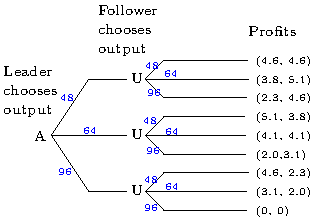
\includegraphics{pics/Stackelberg}
  \end{center}

\end{frame}
\begin{frame}
  \frametitle{Equilibrium}
A strategy is now a complete plan of what action to take whenever a
player has to choose. 
\bigskip

\uncover<2->{So, for $U$, a strategy would consist of three things:
\begin{enumerate}
\item What to do if $A$ chooses 48.
\item What to do if $A$ chooses 64.
\item What to do if $A$ chooses 96.
\end{enumerate}}
\bigskip

\uncover<3->{Since $A$ appears only once in the game tree, a strategy for $A$ is
one of 48, 64, and 96.}
\bigskip

\uncover<4->{A Nash equilibrium consists of a strategy for each player such that no
player can be better off doing something different.}

\end{frame}

\begin{frame}
  \frametitle{Subgame perfect Nash equilibrium}
  We'll actually look for a ``subgame perfect'' equilibrium.

\bigskip
\uncover<2->{A Nash equilibrium is subgame perfect if 

\emph{It is a Nash equilibrium at every subgame.}}

\bigskip
\uncover<3->{That means every player is behaving optimally no matter where we are
on the game tree.}
\end{frame}



\begin{frame}
  \frametitle{The Stackelberg game}
Back to our Stackelberg game:\\
\

  \begin{center}
    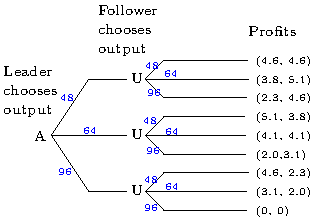
\includegraphics{pics/Stackelberg}
  \end{center}

\end{frame}



\begin{frame}
  \frametitle{What should $A$ do?}
  We have to work backwards (\emph{backwards induction}).
What does $U$ do if $A$ has chosen 48?

  \begin{center}
    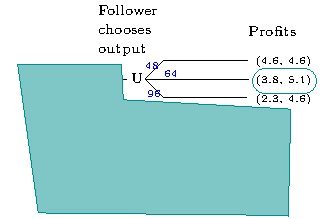
\includegraphics{pics/Stackelberg1}
  \end{center}

\end{frame}


\begin{frame}
  \frametitle{What should $A$ do?}
Continuing our backwards analysis:\\
What does $U$ do if $A$ has chosen 64 instead?

  \begin{center}
    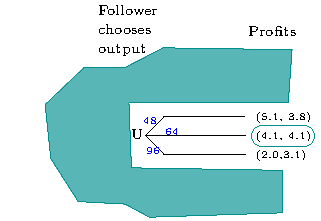
\includegraphics{pics/Stackelberg2}
  \end{center}

\end{frame}

\begin{frame}
  \frametitle{What should $A$ do?}
One more option for $A$::\\
What does $U$ do if $A$ has chosen 96?

  \begin{center}
    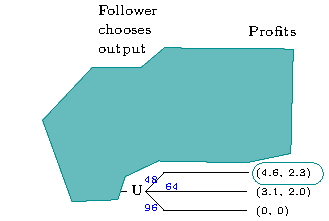
\includegraphics{pics/Stackelberg3}
  \end{center}

\end{frame}

\begin{frame}
  \frametitle{What should $A$ do?}
So depending on what $A$ does, we know what $U$ will (or will not) do
in response when it's his turn.

  \begin{center}
    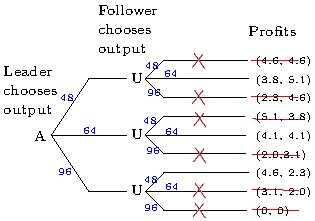
\includegraphics{pics/Stackelberg4}
  \end{center}

\end{frame}

\begin{frame}
  \frametitle{What should $A$ do?}
From $A$'s perspective, we could just get rid of the branches that $U$
won't go down.

  \begin{center}
    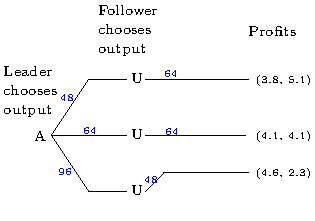
\includegraphics{pics/Stackelberg5}
  \end{center}

\end{frame}

\begin{frame}
  \frametitle{What should $A$ do?}
Now it's clear what $A$'s payoff is depending on what he
chooses. He'll pick the action that gives him the highest profit.

  \begin{center}
    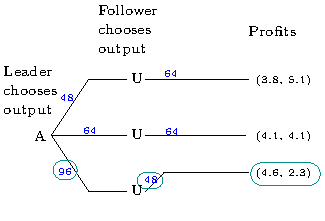
\includegraphics{pics/Stackelberg6}
  \end{center}

\end{frame}


\begin{frame}
  \frametitle{Subgame perfect Nash equilibrium}
  What we found (that $A$ picks 96 and $U$ picks 48) is a
  subgame perfect Nash equilibrium:
\bigskip

\uncover<2->{Why do we care about ``subgame perfection''?}
\bigskip

\uncover<3->{It says that ``off the equilibrium path'' everyone behaves optimally.}
\bigskip

\uncover<4->{In other words, if $A$ picks 64 instead of 96, $U$ will still maximize
his own profits. }

\end{frame}

\begin{frame}
  \frametitle{Is every Nash equilibrium subgame perfect?}
  Remember that both picking 64 was a Nash equilibrium of the
  (simultaneous move version of the) game.
  \bigskip

\uncover<2->{  If $U$ picks the strategy of always picking 64 no matter what $A$
  does, then $A$'s best response is to pick 64.}

  \bigskip

\uncover<3->{  So it's a Nash equilibrium for $U$ to pick 64 no matter what $A$
  does and for $A$ to pick 64.}

\end{frame}

\begin{frame}
  \frametitle{Is it subgame perfect?}
Is it subgame perfect for $A$ to pick 64 and $U$ to \emph{always}
pick 64?

\bigskip
\uncover<2->{Nope. It relies on $U$ doing something that's not optimal for him
``off the equilibrium path'' should $A$ pick 96 instead of 64.}
\uncover<3->{\begin{center}
  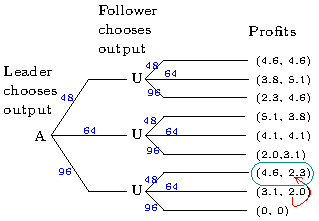
\includegraphics{pics/Stackelberg7}
\end{center}

He'd be better off picking 48 in that case.}
  
\end{frame}

\begin{frame}
  \frametitle{Credibility}
  It seems strange: $U$ would be better off if he could convince $A$
  that he would not do what's optimal for him should $A$ pick 96.

  \bigskip
\uncover<2->{  Essentially, $U$ could threaten $A$ with picking 64 even if $A$ were
  to choose 96. }

  \bigskip
\uncover<3->{  This would only be an equilibrium if $A$ ``believes'' $U$'s threat.}

  \bigskip
\uncover<4->{  If $U$ can't \emph{commit} to 64, then $A$ can call his bluff.}
  \bigskip

\uncover<5
->{  So $U$'s threat to pick 64 isn't \emph{credible}.}

\end{frame}


\begin{frame}
  \frametitle{The dynamic entry game}
  Two firms: incumbent, rival.
\bigskip

\uncover<2->{Incumbent can pay a fee of $b$ to have monopoly rights.}
\bigskip

\uncover<3->{  Incumbent's monopoly profit: 10}
\bigskip

\uncover<4->{Cost of entry for the rival: $F$}
\bigskip

\uncover<5->{Rivals profit if it enters: 4.}
\bigskip

\uncover<6->{Incumbent's profit if rival enters: 4}

\end{frame}

\begin{frame}
  \frametitle{Way easier understand as a game tree}
  \begin{center}
    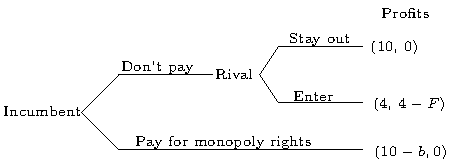
\includegraphics{pics/Entrygame}
  \end{center}

\end{frame}


\begin{frame}
  \frametitle{Subgame perfect equilibrium}
  This will depend on $b$ and $F$.

  \begin{enumerate}
  \item<2-> If $F>4$ obviously rival never enters. So incumbent
    doesn't need to pay for the monopoly rights.
  \item<3-> If $F\leq 4$ then the rival will enter when given a
    chance. So now things depend on $b$:
    \begin{itemize}
    \item<4-> If $b\leq 6$ then the incumbent gets 4 if he doesn't pay
      and $10-b \geq 4$ if he does. So he pays and the rival is kept
      out.
    \item<5-> If $b>6$ then the incumbent gets 4 if he doesn't pay and
      $10-b < 4$ if he does. So he doesn't pay and the rival enters.
    \end{itemize}
  \end{enumerate}
\end{frame}

\begin{frame}
  \frametitle{Auctions}
  Auctions are a common way to sell goods.
  \bigskip

\uncover<2->{  Effectively a game played between bidders: each one picks a bid and
  depending on all of the bids, there's a payoff.
}

  \bigskip
\uncover<3->{  Kinds of auctions:}
  \begin{enumerate}
  \item<4->  English auctions:  bidders raise one another until ``going
    once, going twice, gone.'' 
  \item<5-> Dutch auctions: The ``opposite'' of an English auction. The
    auctioneer starts at a high price and keeps lowering it until
    someone decides to buy.


  \item<6-> Sealed bid auctions: Bidders simultaneously submit bids
    and the highest one wins. Kinds of sealed bid auctions:
    \begin{enumerate}
    \item<7->     \emph{First price auction}: winner pays his bid.
    \item<8-> \emph{Second price auction}: winner pays highest losing bid.
    \end{enumerate}
  \end{enumerate}
  
\end{frame}


\begin{frame}
  \frametitle{Values}
  How people value the good being sold makes a difference in our
  analysis of the auction. 

  \begin{enumerate}
  \item<2-> Private values: each bidder's valuation of the good is
    unrelated to other bidders' valuations. E.g. Art auctions.
  \item<3-> Common values: the value each bidder gets from owning the
    good is the same. But nobody knows exactly what that value
    is but have different estimates. E.g. oil and gas leases.
  \end{enumerate}
\uncover<4->{Most real-world auctions are somewhere between these two.}
\bigskip

\uncover<5->{We'll think about situations where bidders don't know each other
values (or estimates of it in the common value case).}
\end{frame}

\begin{frame}
  \frametitle{Bidding strategies in private value auctions}
  Easiest to analyze: second-price auctions
  \bigskip

\uncover<2->{  \emph{Weakly dominant strategy:} bid your value.}

  \bigskip

\uncover<3->{  No matter what other bidders do, no other strategy can give you a higher payoff!!}

\bigskip
\uncover<4->{The main reason is that your bid only affects whether you win or
not. It does not affect what you pay given that you're winning.}
\end{frame}
\begin{frame}
  \frametitle{Why is it optimal to bid your value?}
  Suppose your value of the good is \$100.
\bigskip

\uncover<2->{If you bid \$100:}
\begin{enumerate}
\item<3-> If the next highest bid, $b$ is less than \$100, you win  the
  auction and your CS is \$($100 - b$).
\item <4-> If the next highest bid is higher than \$100, you lose the
  auction and your CS is 0.
\end{enumerate}

\end{frame}

\begin{frame}
  \frametitle{Why you shouldn't bid less than \$100}
Suppose you bid less than \$100, say \$90.
\begin{enumerate}
\item <2-> If the next highest bid, $b$ is less than \$90, you win and
  your CS is \$$(100-b)$ --- the same as if you bid \$100.
\item<3-> If the next highest bid is between \$90 and \$100, you
  lose the auction and your CS is 0 --- lower than if you bid \$100.
\item<4-> If the next highest bid is higher \$100, you
lose the auction and your CS is 0  --- the same as if you bid \$100.
\end{enumerate}

\uncover<5->{So you're never worse off and sometimes better off bidding \$100 than \$90.}
\end{frame}

\begin{frame}
  \frametitle{Why you shouldn't bid more than \$100}
Suppose you bid less than \$100, say \$110.
\begin{enumerate}
\item <2-> If the next highest bid, $b$ is less than \$100, you win and
  your CS is \$$(100-b)$ --- the same as if you bid \$100.
\item<3-> If the next highest bid, $b$  is between \$100 and \$110, you win
  and  your CS is \$$(100-b) < 0$ --- lower than if you bid \$100.
\item<4-> If
 the next highest bid is higher \$110, you
lose the auction and your CS is 0  --- the same as if you bid \$100.
\end{enumerate}

\uncover<5->{ So you're never worse off and sometimes better off bidding \$100 than \$110.}
\end{frame}

\begin{frame}
  \frametitle{English auctions}
Second price sealed-bid auction  is equivalent to an English auction! Why?


\bigskip
\uncover<2->{ When do you stop raising other bidders?}
\bigskip

\uncover<3->{ When the current bid meets your value!}

\bigskip
\uncover<4->{ So, the person with the highest value pays the second highest value:
that's the price at which all but one bidder drops out.}
 
\end{frame}


\begin{frame}
  \frametitle{Equivalence of auctions}
  Do you bid your valuation in a first price auction?

\bigskip
\uncover<2->{ Of course not. That gives you a guaranteed CS of \$0.}

  \bigskip
\uncover<3->{   You will \emph{shave} your bid and bid less than your valuation.}

\bigskip
\uncover<4->{ Same goes for the Dutch auction.}

\bigskip
\uncover<5->{ How much you \emph{shave}  your bid depends on the statistical
distribution of others' values. }

\bigskip
\uncover<6->{ \emph{The revenue equivalence theorem:} The auctioneer gets the same
``expected'' profit no matter what auction he uses (as long as the
person who values it most wins the good).}
 
\end{frame}

\begin{frame}
  \frametitle{Common value auctions}
  Each bidder has an estimate of how valuable the good is.

\medskip
\uncover<2->{ Cannot know the true value until it's yours.}
\medskip

\uncover<3->{ The person with the highest bid is most likely the person who has the
highest \emph{estimate} of the good's true value.}

\medskip
\uncover<4->{ The highest estimate is almost always higher than the true value.}
\medskip

\uncover<5->{ So the winner is usually disappointed to find that the good is worse
than he anticipated.}

\medskip
\uncover<6->{ Bids in these kind of auctions are usually low because people foresee
this ``winner's curse.''}

\medskip
\uncover<7->{ Auctioneer can do better to have information be revealed as bidding
proceeds: English auction would be better than a second price auction.}


\end{frame}


\end{document}



